\documentclass[
  11pt,
  letterpaper,
   addpoints,
   answers
  ]{exam}

% Carga el preámbulo localizado en la carpeta superior
\NeedsTeXFormat{LaTeX2e}[2023/04/30]

% Provide the name of your page, the date it was last updated, and a comment about what it's used for
\ProvidesPackage{../exercise-preamble}[2023/04/30 Prof. Cassanelli custom LaTeX style]

% \usepackage{printlen}
% \uselengthunit{in}\printlength{\textwidth}

% PACKAGES
\usepackage[dvipsnames]{xcolor}

\usepackage{graphicx}
\graphicspath{{../figures}}
\usepackage{amsmath,amsthm,amssymb,mathtools,mathrsfs}
\usepackage{commath}
\usepackage{upgreek}
\usepackage{cancel}
\usepackage{enumerate}
\usepackage[font=small]{caption}
\usepackage[normalem]{ulem}
\usepackage{steinmetz}
\usepackage{enumitem}
\usepackage[left=1.5cm, right=1.5cm, top=1cm]{geometry}
\usepackage{wrapfig}

% REFERENCES AND OTHERS
\usepackage{../aas_macros}
\usepackage{natbib}
\bibpunct{(}{)}{;}{a}{}{,}

\usepackage{tikz}
\usepackage{tikz-3dplot}
\usepackage{circuitikz}
\usepackage{pgfplots}
\pgfplotsset{compat=1.15}
\usepgfplotslibrary{smithchart}
\usetikzlibrary{
  decorations.pathmorphing,
  decorations.markings,
  calc,
  patterns,
  decorations,
  angles,
  quotes,
  ext.topaths.arcthrough,
  shapes
  }

\usepackage{siunitx}
\sisetup{
    range-phrase=\text{--},
    range-units=single,
    separate-uncertainty=true,
    print-unity-mantissa=false
    }
\DeclareSIUnit{\gauss}{G}
\DeclareSIUnit{\jansky}{Jy}

\newcommand{\iu}{\mathrm{i}\mkern1mu}
\newcommand{\ju}{\mathrm{j}\mkern1mu}
\newcommand{\euler}{\mathrm{e}}
\newcommand{\exponential}[1]{\mathrm{exp}\left[#1\right]}
\newcommand{\uvec}[1]{\widehat{\mathbf{#1}}}
\newcommand{\uvecs}[1]{\boldsymbol{\widehat{#1}}}
\newcommand{\bvec}[1]{\boldsymbol{\mathcal{#1}}}

\usepackage{hyperref}
\hypersetup{
    % bookmarks=true,
    unicode=true,
    pdftoolbar=true,
    pdfmenubar=true,
    pdffitwindow=false,
    pdfstartview={FitH},
    pdftitle={EL3103},
    pdfauthor={Tomas Cassanelli},
    pdfcreator={Tomas Cassanelli},
    pdfnewwindow=true,
    colorlinks=true,
    linkcolor=Violet,
    citecolor=Violet,
    urlcolor=Violet
    }

% Exam document class
\renewcommand{\figurename}{Figura}
\renewcommand{\tablename}{Cuadro}
\pagestyle{empty}

\usepackage[spanish]{cleveref}

\crefname{question}{\protect{pregunta}}{\protect{preguntas}}
\Crefname{question}{\protect{Pregunta}}{\protect{Preguntas}}
\creflabelformat{question}{#2{#1}#3}

\renewcommand{\solutiontitle}{\noindent\textbf{Solución:}\par\noindent}
\bracketedpoints
\pointname{~puntos}

\endinput

% Paquetes locales
\usepackage{float}
\usepackage{booktabs} % para \toprule, \midrule, \bottomrule

% Macros locales
\newcommand{\Rel}{\mathfrak{R}} % símbolo para la reluctancia

\begin{document}

\noindent
\begin{minipage}{0.47\textwidth}

\includegraphics[width=\textwidth]{../fcfm_die}
\end{minipage}
\begin{minipage}{0.53\textwidth}
\begin{center}
\large\textbf{Análisis de Sistemas Dinámicos y Estimación} (EL3204-1) \\
\large\textbf{Ejercicio 1} \\
\normalsize Prof.~ Marcos Orchard - Sebastián Espinosa.\\
\normalsize Prof.~Aux.~Erik Sáez
\end{center}
\end{minipage}

\vspace{0.5cm}
\noindent\fbox{%
  \parbox{\dimexpr\linewidth-2\fboxsep-2\fboxrule\relax}{%
    	\textbf{Instrucciones:} La tarea se puede realizar en parejas con un plazo máximo hasta el 30 de septiembre; no se aceptarán atrasos. El formato deberá ser entregada en físico (letra legible o \LaTeX{}), además de entrega virtual de los códigos que utilicen.
  }%
}

\vspace{.85cm}

\begin{questions}
    %%%%%%%%%%%%%%%%%%%%%%%%%%%
    \question \section*{Modelo simplificado de un relé}

Considere el sistema electromecánico de la figura~\ref{fig:relay}, que modela de forma simplificada el funcionamiento de un relé. Consta de un núcleo de hierro de sección transversal $A$ en el cual se induce flujo magnético mediante una bobina de $N$ vueltas. Para este estudio, usted podrá modificar el voltaje de excitación $e(t)$. Como caso motivador, se está diseñando y validando un relé para accionar la válvula neumática de la pinza de un brazo robótico didáctico; se busca un cierre rápido y repetible (\textless{}60~ms) con bajo consumo. Por ello se analizará cómo el entrehierro modula $L(x)$, la fuerza de atracción y el tiempo de conmutación.

\begin{figure}[h!]
  \centering
  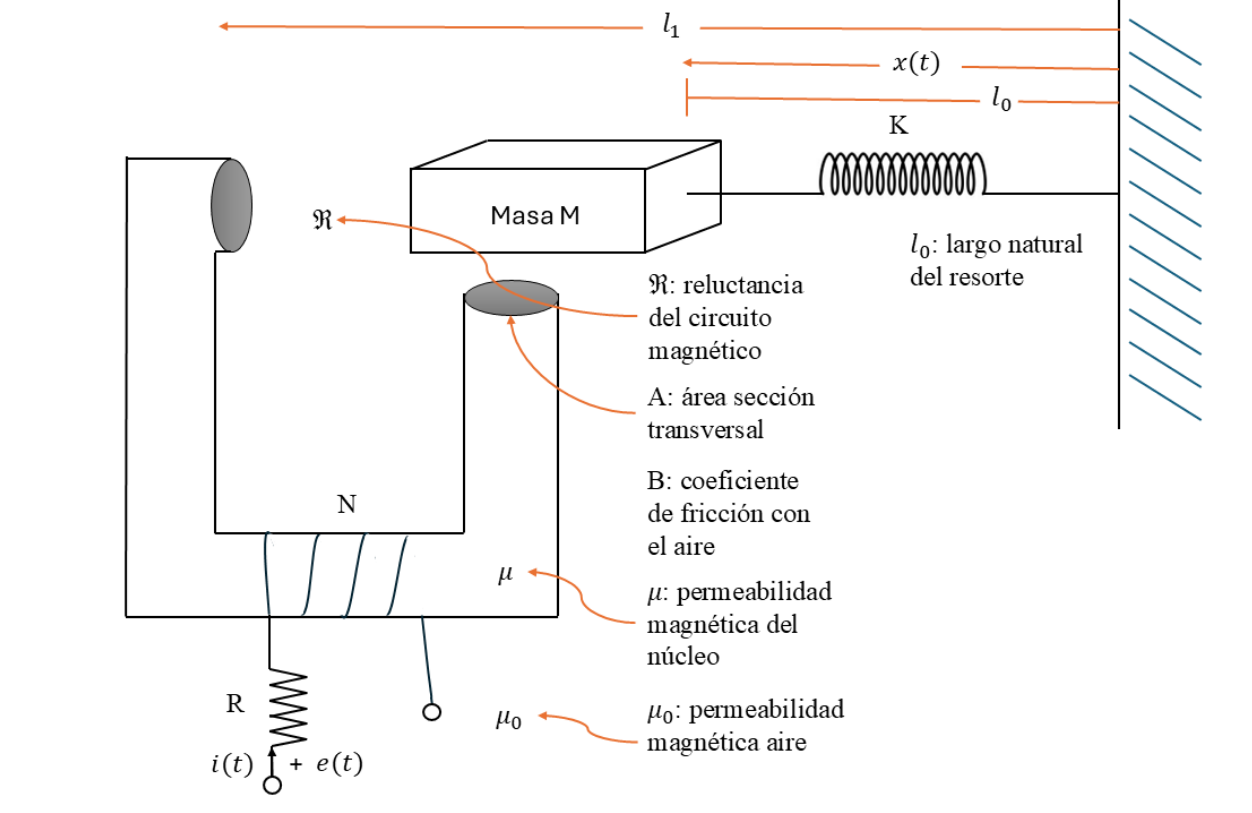
\includegraphics[width=0.8\textwidth,keepaspectratio]{Ejercicio_1_1}
  \caption{Modelo simplificado del funcionamiento de un relé.}
  \label{fig:relay}
\end{figure}

Los parámetros del sistema se presentan en la Tabla~\ref{tab:variables}.

\begin{table}[h!]
  \centering
  \caption{Variables y parámetros del sistema}
  \label{tab:variables}
  \small
  \begin{tabular}{@{}l p{9.5cm} c@{}}
    \toprule
    \textbf{Variable/Parámetro} & \textbf{Definición} & \textbf{Unidad} \\
    \midrule
    $x(t)$      & Posición de la armadura móvil entre $l_0$ y $l_1$ & m \\
    $i(t)$      & Corriente por la bobina                           & A \\
    $L(x)$      & Inductancia de la bobina                          & H \\
  $\Rel$      & Reluctancia del circuito magnético                & A/Wb (1/H) \\
    $e(t)$      & Voltaje en la bobina                              & V \\
    $M$         & Masa de la pieza                                  & kg \\
    $K$         & Coeficiente de rigidez del resorte                & N/m \\
    $B$         & Coeficiente de fricción viscosa del aire          & N/(m/s) \\
    $R$         & Resistencia eléctrica de la bobina                & $\Omega$ \\
    $A$         & Área de la sección transversal del núcleo         & m$^2$ \\
    $\mu$       & Permeabilidad magnética del núcleo                & H/m \\
    $\mu_0$     & Permeabilidad magnética del aire                  & H/m \\
    $N$         & Número de espiras de la bobina                    & -- \\
    \bottomrule
  \end{tabular}
\end{table}

\medskip
Para un mejor contexto de la tarea, considere la figura~\ref{fig:core}.

\begin{figure}[h!]
  \centering
  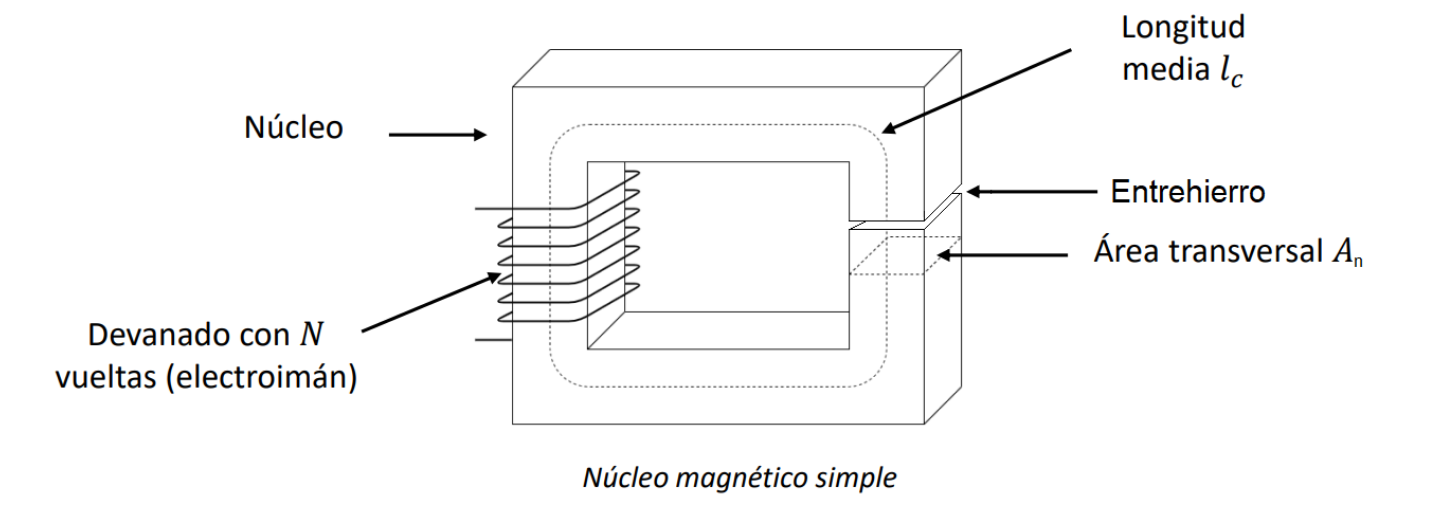
\includegraphics[width=0.85\textwidth,keepaspectratio]{Ejercicio_1_2}
  \caption{Núcleo simple}
  \label{fig:core}
\end{figure}

Por definición, la fuerza del campo magnético generada por la inductancia es
\begin{equation*}
  F_m = N \cdot i(t).
\end{equation*}
Luego, por ley de Ampere, se debe cumplir que para un loop cerrado:
\begin{align*}
  N \cdot i
  &= H_n \cdot l_n + H_g \cdot l_g \\
  &= \frac{B_n}{\mu} \cdot l_n + \frac{B_g}{\mu_0} \cdot l_g .
\end{align*}
Ahora bien, el flujo magnético es la integral de superficie transversal sobre el campo magnético, es decir,
\begin{equation*}
  \int B_{n,g}\, \mathrm{d}s = \phi,
\end{equation*}
Luego, como el campo magnético no varía de forma transversal en el núcleo:
\begin{equation*}
  B_{n,g} = \frac{\phi}{A_n}.
\end{equation*}
Luego,
\begin{align*}
  N \cdot i
  &= \frac{\phi}{A_n \mu} \cdot l_n + \frac{\phi}{A_n \mu_0} \cdot l_g \\
  &= \phi\!\left(\frac{l_n}{A_n \mu} + \frac{l_g}{A_n \mu_0}\right).
\end{align*}

Donde $B_n$ y $l_n$ corresponden al campo magnético y el largo promedio del núcleo respectivamente. Por otra parte, $B_g$ y $l_g$ corresponden al campo magnético del vacío y el largo del entrehierro.

La reluctancia $\Rel$ corresponde a un parámetro que cuantifica la resistencia de un material al flujo magnético. Depende de la permeabilidad del material magnético ($\mu_m$), el área de la sección transversal ($A$) y la longitud del material ($l$), es decir:
\begin{equation}
  \Rel = \frac{l}{A\,\mu_m}.
  \label{eq:reluctancia}
\end{equation}
Por tanto,
\begin{align*}
  N\,i &= \phi\,(\Rel_n + \Rel_g), \\
  \phi &= \frac{N\,i}{\Rel_n + \Rel_g}.
\end{align*}

El voltaje en la bobina debe satisfacer las siguientes igualdades
\begin{equation*}
  V_{\text{bobina}} = L\,\frac{\mathrm{d}i}{\mathrm{d}t}
  = N\,\frac{\mathrm{d}\Phi}{\mathrm{d}t}.
\end{equation*}
Si se integra la ecuación anterior respecto al tiempo:
\begin{equation*}
  L\,i = N\,\Phi.
\end{equation*}
Entonces,
\begin{equation*}
  L\,i = N\, \frac{N\, i}{\Rel_n + \Rel_g}
\end{equation*}
Luego, definiendo $\Rel_{\text{total}} = \Rel_n + \Rel_g$ y despejando $L$:
\begin{equation}
  L = \frac{N^2}{\Rel}
  \label{eq:LfromR}
\end{equation}

\medskip
La ecuación~\eqref{eq:LfromR} (y, por consecuencia, \eqref{eq:reluctancia}) será útil. Es recomendable tratar $L$ como función de la longitud del tramo donde la reluctancia no es despreciable.

En el problema de la tarea planteado hay básicamente dos tipos de reluctancia. Una es debida a la oposición al paso del flujo magnético en el camino de aire; la otra se debe a la oposición al flujo en el núcleo de hierro. Para estos fines, considere que el hierro es un muy buen conductor de flujo magnético comparado con el aire y que la pieza móvil también es de hierro. En base a este problema, se requiere estudiar el movimiento y velocidad de la pieza de masa $M$ además de la corriente que se inyecta al sistema. Para ello, usted debe contestar las preguntas planteadas en las siguientes páginas.

\vspace{0.5cm}
\noindent\fbox{\textbf{P1.- Modelamiento matemático}}

\begin{enumerate}
  \item Establezca de forma clara todas las hipótesis simplificatorias del sistema. Considere que la Figura~\ref{fig:core} no tiene errores y, por tanto, si considera que falta algún dato o parámetro indique cómo abordará esto para que el modelo tenga sentido. Además, se aconseja investigar sobre transformadores ideales.

  \item Formule el modelo matemático. Para ello deberá encontrar dos ecuaciones; una para la parte eléctrica del sistema y la otra para la parte mecánica del mismo. \emph{Hint}: la fuerza magnética interactúa con la pieza móvil según $F_m = \tfrac{1}{2} i^2\, \dfrac{\mathrm{d}L}{\mathrm{d}x}$. Además, si el valor $L$ de una inductancia varía con el tiempo a través de una función $g(t)$, entonces, el voltaje en esa inductancia será $V_{\text{ind}} = \dfrac{\mathrm{d}}{\mathrm{d}t}\big[L\big(g(t)\big)\, i(t)\big]$.

  \item En base al contexto del problema, indique las variables que corresponden a la/s entrada/s, salida/s y variable/s de estado del sistema. Replantee el modelo como un sistema matricial de la forma $\dot{\vec{X}}(t) = \vec{F}\big(\vec{X}(t), u(t)\big)$ con su respectiva salida $\vec{Y}(t) = C \cdot \vec{X}(t)$, donde $\vec{X}(t)$ representa el vector de estados, $C$ la matriz de salida y $u(t)$ la/s entrada/s al sistema.

  \item Encuentre el/los estado/s de equilibrio del sistema no lineal.

  \item Encuentre las ecuaciones del/los punto/s de operación que asegura que la pieza móvil esté en una posición arbitraria $x_0$. Luego, exprese una única ecuación que involucre la posición de la pieza móvil y la entrada $u_0(t)$ (no es necesario despejar la posición de la pieza móvil).
\end{enumerate}

\vspace{0.5cm}
\noindent\fbox{\textbf{P2.- Linealización-Laplace-MTE}}

\begin{enumerate}
  \item Linealice el sistema planteado en la pregunta anterior en torno a un punto de operación arbitrario $(\vec{X}(t_0), u(t_0))$ con tal de obtener la expresión $\dot{\vec{X}} = A \cdot \vec{X} + B \cdot u$, donde $A$ es la matriz de estado y $B$ la matriz de entrada.

  \item Considere el sistema linealizado del primer punto. Evalúe el sistema en torno al estado de equilibrio que usted considere pertinente según lo que encontró en P1.4. \textbf{Importante:} Para las siguientes preguntas se considerará este sistema en particular.

  \item Obtenga la MTE del sistema linealizado en torno al punto de equilibrio.

  \item Obtenga la función de transferencia del sistema linealizado en torno al punto de equilibrio.
\end{enumerate}

\vspace{0.5cm}
\noindent\fbox{\textbf{P3.- Determinación de estados}}

\begin{enumerate}
  \item Encuentre el/los estado/s cero del sistema linealizado en torno al punto de equilibrio.

  \item Encuentre el/los estado/s tierra del sistema linealizado en torno al punto de equilibrio.
\end{enumerate}

\vspace{0.5cm}
\noindent\fbox{\textbf{P4.- Polos-Respuesta al impulso-RESC-RENC}}

\begin{enumerate}
  \item Encuentre los polos del sistema linealizado en torno al punto de equilibrio.

  \item Utilizando la función de transferencia, encuentre la respuesta al impulso en el dominio del tiempo del sistema linealizado en torno al punto de equilibrio.

  \item Encuentre la RESC para el sistema linealizado en torno al punto de equilibrio.

  \item Encuentre la RENC para condiciones iniciales arbitrarias para el sistema linealizado en torno al punto de equilibrio.

  \item Exprese la solución completa del sistema linealizado en torno al punto de equilibrio.
\end{enumerate}

\vspace{0.5cm}
\noindent\fbox{\textbf{P6.- Simulaciones Matlab}}

\begin{enumerate}
  \item Considere el contexto de la parte 5 de la pregunta 1. Grafique en un mismo gráfico las fuerzas eléctrica y mecánica en función de la posición $x(t)$ de la pieza móvil entre el rango $[l_0, l_1]$ (con el paso que usted estime pertinente). Indique la posición y corriente que asegura equilibrio en el sistema considerando que el voltaje es $e(t)) = 2~[\text{V}]$. Para ello considere los siguientes casos de la Tabla~\ref{tab:casos-corriente}:

  \begingroup
  \renewcommand{\tablename}{Tabla}
  \begin{table}[H]
    \centering
    \caption{Casos de corriente}
    \label{tab:casos-corriente}
    \small
    \begin{tabular}{|c|c|}
      \hline
      	extbf{Caso} & $I_0$ [A] \\
      \hline
      a & 1 \\
      \hline
      b & 2 \\
      \hline
      c & 3 \\
      \hline
    \end{tabular}
  \end{table}
  \endgroup

  \item Simule el sistema y analice la respuesta completa del sistema de tiempo continuo frente a un escalón unitario y señales sinusoidales con 2 frecuencias distintas, considerando al menos dos condiciones iniciales en todos los casos. Las frecuencias de las señales sinusoidales y las componentes que definen condiciones iniciales deben generarse mediante realizaciones de variables aleatorias con distribución uniforme, cuyo soporte debe ser debidamente reportado. Analice sus resultados y concluya cómo afectan las condiciones iniciales y las diferentes entradas al sistema.

  \item Implemente el observador anteriormente diseñado, y simule el sistema observado para entradas y condiciones iniciales generados bajo el mismo criterio que la pregunta anterior. Debe graficar el error en el observador para cada uno de los estados, además de las salidas del sistema original y del sistema observado. Comente sobre sus resultados.
\end{enumerate}

\vspace{0.5cm}
\noindent\fbox{\textbf{P5.- Estabilidad-Controlabilidad y observabilidad}}

\begin{enumerate}
  \item Determine la estabilidad del sistema linealizado en torno al punto de equilibrio.

  \item Determine si el sistema es controlable.

  \item Considere ahora que $C = [111]$. Determine si el sistema es observable.

  \item Considere ahora que $C = [111]$. Diseñe un observador de Luenberger para el sistema a tiempo continuo. Como criterio de diseño, para elegir los polos del observador, considere que los polos del observador deben ser, al menos, 3 veces más negativos que todos los polos del sistema original. Puede dejar expresadas las ecuaciones (3) para resolver el problema (no es necesario que lo resuelva).
\end{enumerate}

\vspace{0.75cm}
\begin{center}
Para las siguientes preguntas considere estos valores para los parámetros del problema 2:

\medskip
	extbf{Tabla 2: Parámetros dados.}
\end{center}

\begin{table}[h!]
  \centering
  \begin{tabular}{@{}c c@{}}
    	oprule
    	extbf{Parámetro} & \textbf{Valor} \\
    \midrule
    $l_1$ & $0.03\,[\mathrm{m}]$ \\
    $l_0$ & $0.02\,[\mathrm{m}]$ \\
    $N$   & $200$ espiras \\
    $a$   & $0.0001\,[\mathrm{m}^2]$ \\
    $\mu_0$ & $4\pi \times 10^{-7}\,[\mathrm{H/m}]$ \\
    $K$   & $0.01\,[\mathrm{N/m}]$ \\
    $B$   & $0.00000001\,[\mathrm{N/(m/s)}]$ \\
    \bottomrule
  \end{tabular}
\end{table}
\end{questions}
\end{document}